\chapter{Deep Media Processing}
\label{chap:deep-media}

Long-form video is structurally unlike every other source type AI Compass ingests: a research preprint or a government notice arrives as text the enrichment agent can read directly, but a video's substantive content is locked inside an audio track until something turns it into text. This chapter documents how the pipeline acquires a transcript for every ingested YouTube video, how it falls back to local speech-to-text when no caption track exists, how it copes with videos long enough that a single enrichment pass over the full transcript is neither practical nor within the system's own truncation limit, and how the resulting per-chapter summaries are exposed differently to Free and Pro viewers without duplicating the underlying computation.

\section{Caption Retrieval and STT Fallback}
\label{sec:deep-media-captions}

Every scraped YouTube video first attempts a caption-based transcript rather than committing directly to transcription. The caption-fetch step tries three sources in a fixed priority order: a manually created English caption track, if the uploader supplied one; failing that, an auto-generated English caption track; and failing that, an auto-generated caption track in any other language, machine-translated to English. This ordering reflects a simple accuracy hierarchy (a human-authored caption is trusted over a machine-generated one in the same language, which is in turn trusted over a machine-generated caption that has passed through an additional translation step), and it means the majority of videos that any caption track at all, in any language, never need to reach the transcription stage described in Section~\ref{sec:deep-media-transcription}.

When none of the three caption sources yields anything, the video is not dropped or deferred: it is still inserted into the corpus, with its content field left empty, and a speech-to-text job is queued against it in a dedicated \texttt{stt\_jobs} table with status \texttt{queued}. Keeping the video row in place rather than withholding it until a transcript exists means the item can already participate in title-only discovery and does not silently vanish from the pipeline's bookkeeping while transcription is pending.

An STT job moves through five possible states over its lifetime: \texttt{queued}, \texttt{running}, \texttt{completed}, \texttt{failed}, and \texttt{skipped\_too\_long} (the last of these is produced by the duration gate described in Section~\ref{sec:deep-media-transcription}, not by a transcription failure). The dispatch phase that hands queued jobs off to a Celery worker is written specifically to avoid a race between the database and the task queue: it claims a batch of queued jobs by flipping their status to \texttt{running} and \emph{committing that state change} before it calls the worker task that will actually perform the transcription. This ordering is deliberate rather than incidental: if the dispatch phase instead queued the worker task first and updated the row's status afterward, a worker could in principle start executing before the status flip was visible to it, and look up a row that still read \texttt{queued} even though it was already being processed. Committing the state transition first closes that window: by the time a worker is invoked at all, the row it will act on is guaranteed to already show \texttt{running} to any process that queries it.

\section{Transcription}
\label{sec:deep-media-transcription}

Before any audio is downloaded, the transcription stage runs a metadata-only duration probe against the video, which costs nothing beyond a lookup and requires no audio transfer. The probed duration is checked against a fixed ceiling of 10{,}800 seconds, three hours. A video at or above that ceiling is marked \texttt{skipped\_too\_long} immediately, without its audio ever being pulled; the ceiling exists precisely so that an unusually long recording (a multi-hour livestream re-upload, for instance) cannot consume disproportionate transcription time or storage for a single item.

For every video under the ceiling, audio is downloaded with \texttt{yt-dlp} and transcribed with \texttt{faster-whisper}, using the \texttt{distil-large-v3} distilled Whisper checkpoint as the default model, overridable through an environment variable if a different checkpoint is preferred for a given deployment. The transcription runs entirely on CPU, using int8 quantization; no GPU is used or required anywhere in this path. This matters operationally: it means the speech-to-text capability does not impose a GPU-hosting requirement on the deployment described in Chapter~9, at the cost of transcription taking noticeably longer than the underlying audio's own duration.

That cost is quantified by a genuine measurement recorded directly in the transcription service's own source as a dated code comment, not merely asserted in passing: a real 1{,}013-second (16.9-minute) video was transcribed in 1{,}778 seconds (29.6 minutes) on the development machine's CPU, which works out to approximately 1.76 times real time: that is, transcription took about 1.76 times as long as the video it was transcribing, running slower than real time rather than faster. It is important to state precisely what this figure is and is not. It is one measured data point, taken once, on one specific piece of development hardware, using the default model and quantization settings; it is not a formal benchmark suite, it was not repeated across multiple videos or machines to establish a distribution, and it should not be read as a guarantee of throughput on any other hardware, video length, or content type. Presented with that caveat, it is nonetheless a legitimate and useful figure: it establishes that CPU-only transcription at this model size is well within the range of "eventually finishes in a reasonable multiple of the video's own length" rather than being impractically slow, which is the property that makes running speech-to-text without a GPU a defensible engineering choice for this system rather than a corner cut for lack of one.

\section{Long-Video Chaptering}
\label{sec:deep-media-chaptering}

Whether a transcript originates from a real caption track or from the speech-to-text stage of Section~\ref{sec:deep-media-transcription}, both sources are normalized into the same \texttt{transcript\_segments} representation: a list of objects, each carrying a \texttt{start} time, a \texttt{duration}, and a \texttt{text} field. This shared shape is what allows a single piece of downstream chunking code to operate on either kind of transcript without a conditional branch distinguishing "captioned" from "transcribed" videos: from the chaptering logic's point of view, a caption-sourced and an STT-sourced transcript are indistinguishable inputs.

Videos at or above 1{,}200 seconds (twenty minutes) in duration are treated differently from shorter ones: rather than being summarized in a single pass, they are split into chunks of approximately 600 seconds (ten minutes) each. Chunk boundaries are never placed in the middle of a transcript segment; they are snapped to the nearest whole segment boundary, so that no individual caption or STT line is ever split across two chunks. If the final chunk produced by this process would run under 90 seconds, a short trailing remainder left over after the preceding whole-chunk divisions, it is merged into the previous chunk instead of being kept as its own undersized chunk, avoiding a chapter so short it would carry essentially no independent content.

Each chunk is then summarized independently: one Groq call per chunk produces that chunk's own chapter title and summary. This is the "map" half of a map-reduce structure. The "reduce" half concatenates the resulting chapter summaries, each prefixed with its timestamp, into a single combined text, and passes that combined text through the same content-enrichment agent used for every other ingested item (the one described in Chapter~5). This routing choice is deliberate and solves a real problem: Chapter~5 documents a 10{,}000-character truncation applied to content before enrichment, and a long video's raw transcript is exactly the kind of content most likely to exceed that limit by a wide margin. By enriching the concatenated \emph{chapter summaries} rather than the raw transcript, the reduce step operates on a much shorter, already-condensed text that is unlikely to hit the truncation limit at all, so the one part of the system most exposed to that limitation is precisely the part that ends up routed around it, rather than being the part most damaged by it.

\section{Entitlement Gating}
\label{sec:deep-media-entitlements}

Chapter-level video summaries are gated behind a Pro-only feature flag, \texttt{deep\_video\_summaries}. It is important to be precise about exactly what this flag controls, because it is narrower than it might first appear: it gates only the \emph{display} of a chapter's title and summary text on the video detail page. It does not gate the underlying computation described in Section~\ref{sec:deep-media-chaptering}: the chunking, the per-chunk map step, and the reduce-step enrichment all run for every qualifying video regardless of which plan any particular eventual viewer holds, because that computation happens once, at ingestion time, for the corpus as a whole, before any specific viewer's request exists.

The consequence, confirmed directly in both the pipeline code that produces chapters and the Django API view that serves video detail pages to the frontend, is that a Free-tier viewer is shown the correct number of chapters the video was divided into, but with each chapter's title and summary text blanked out rather than the chapter itself being omitted. This is a locked preview, not a vanished section: the viewer can see that the video has, say, four chapters and where they fall in the timeline, which is enough to convey that deeper structure exists and to motivate an upgrade, without disclosing the Pro-only content itself.

\section{Pipeline Summary}
\label{sec:deep-media-summary}

Figure~\ref{fig:deep-media} draws together the stages covered in this chapter into a single pipeline view. A newly scraped YouTube video first passes through caption retrieval (Section~\ref{sec:deep-media-captions}), trying manual English, then auto-generated English, then translated captions in that order; if all three fail, the video is inserted with empty content and an STT job is queued rather than the item being withheld. The STT dispatch phase claims queued jobs with a commit-before-dispatch ordering that removes the race between the database and the worker queue, after which the duration gate of Section~\ref{sec:deep-media-transcription} either short-circuits an over-long video to \texttt{skipped\_too\_long} or proceeds to audio download and CPU-based \texttt{faster-whisper} transcription. Whatever transcript results (captioned or transcribed, both normalized to the same \texttt{transcript\_segments} shape) feeds the duration check in Section~\ref{sec:deep-media-chaptering}: short videos are enriched directly, while videos of twenty minutes or more are chunked, mapped to per-chunk chapter summaries, and reduced through the shared enrichment agent. Finally, Section~\ref{sec:deep-media-entitlements}'s entitlement check is applied only at serving time, on the already-computed chapters, to decide whether a given request's viewer sees the chapter text or a locked preview of it.

\begin{figure}[htbp]
\centering
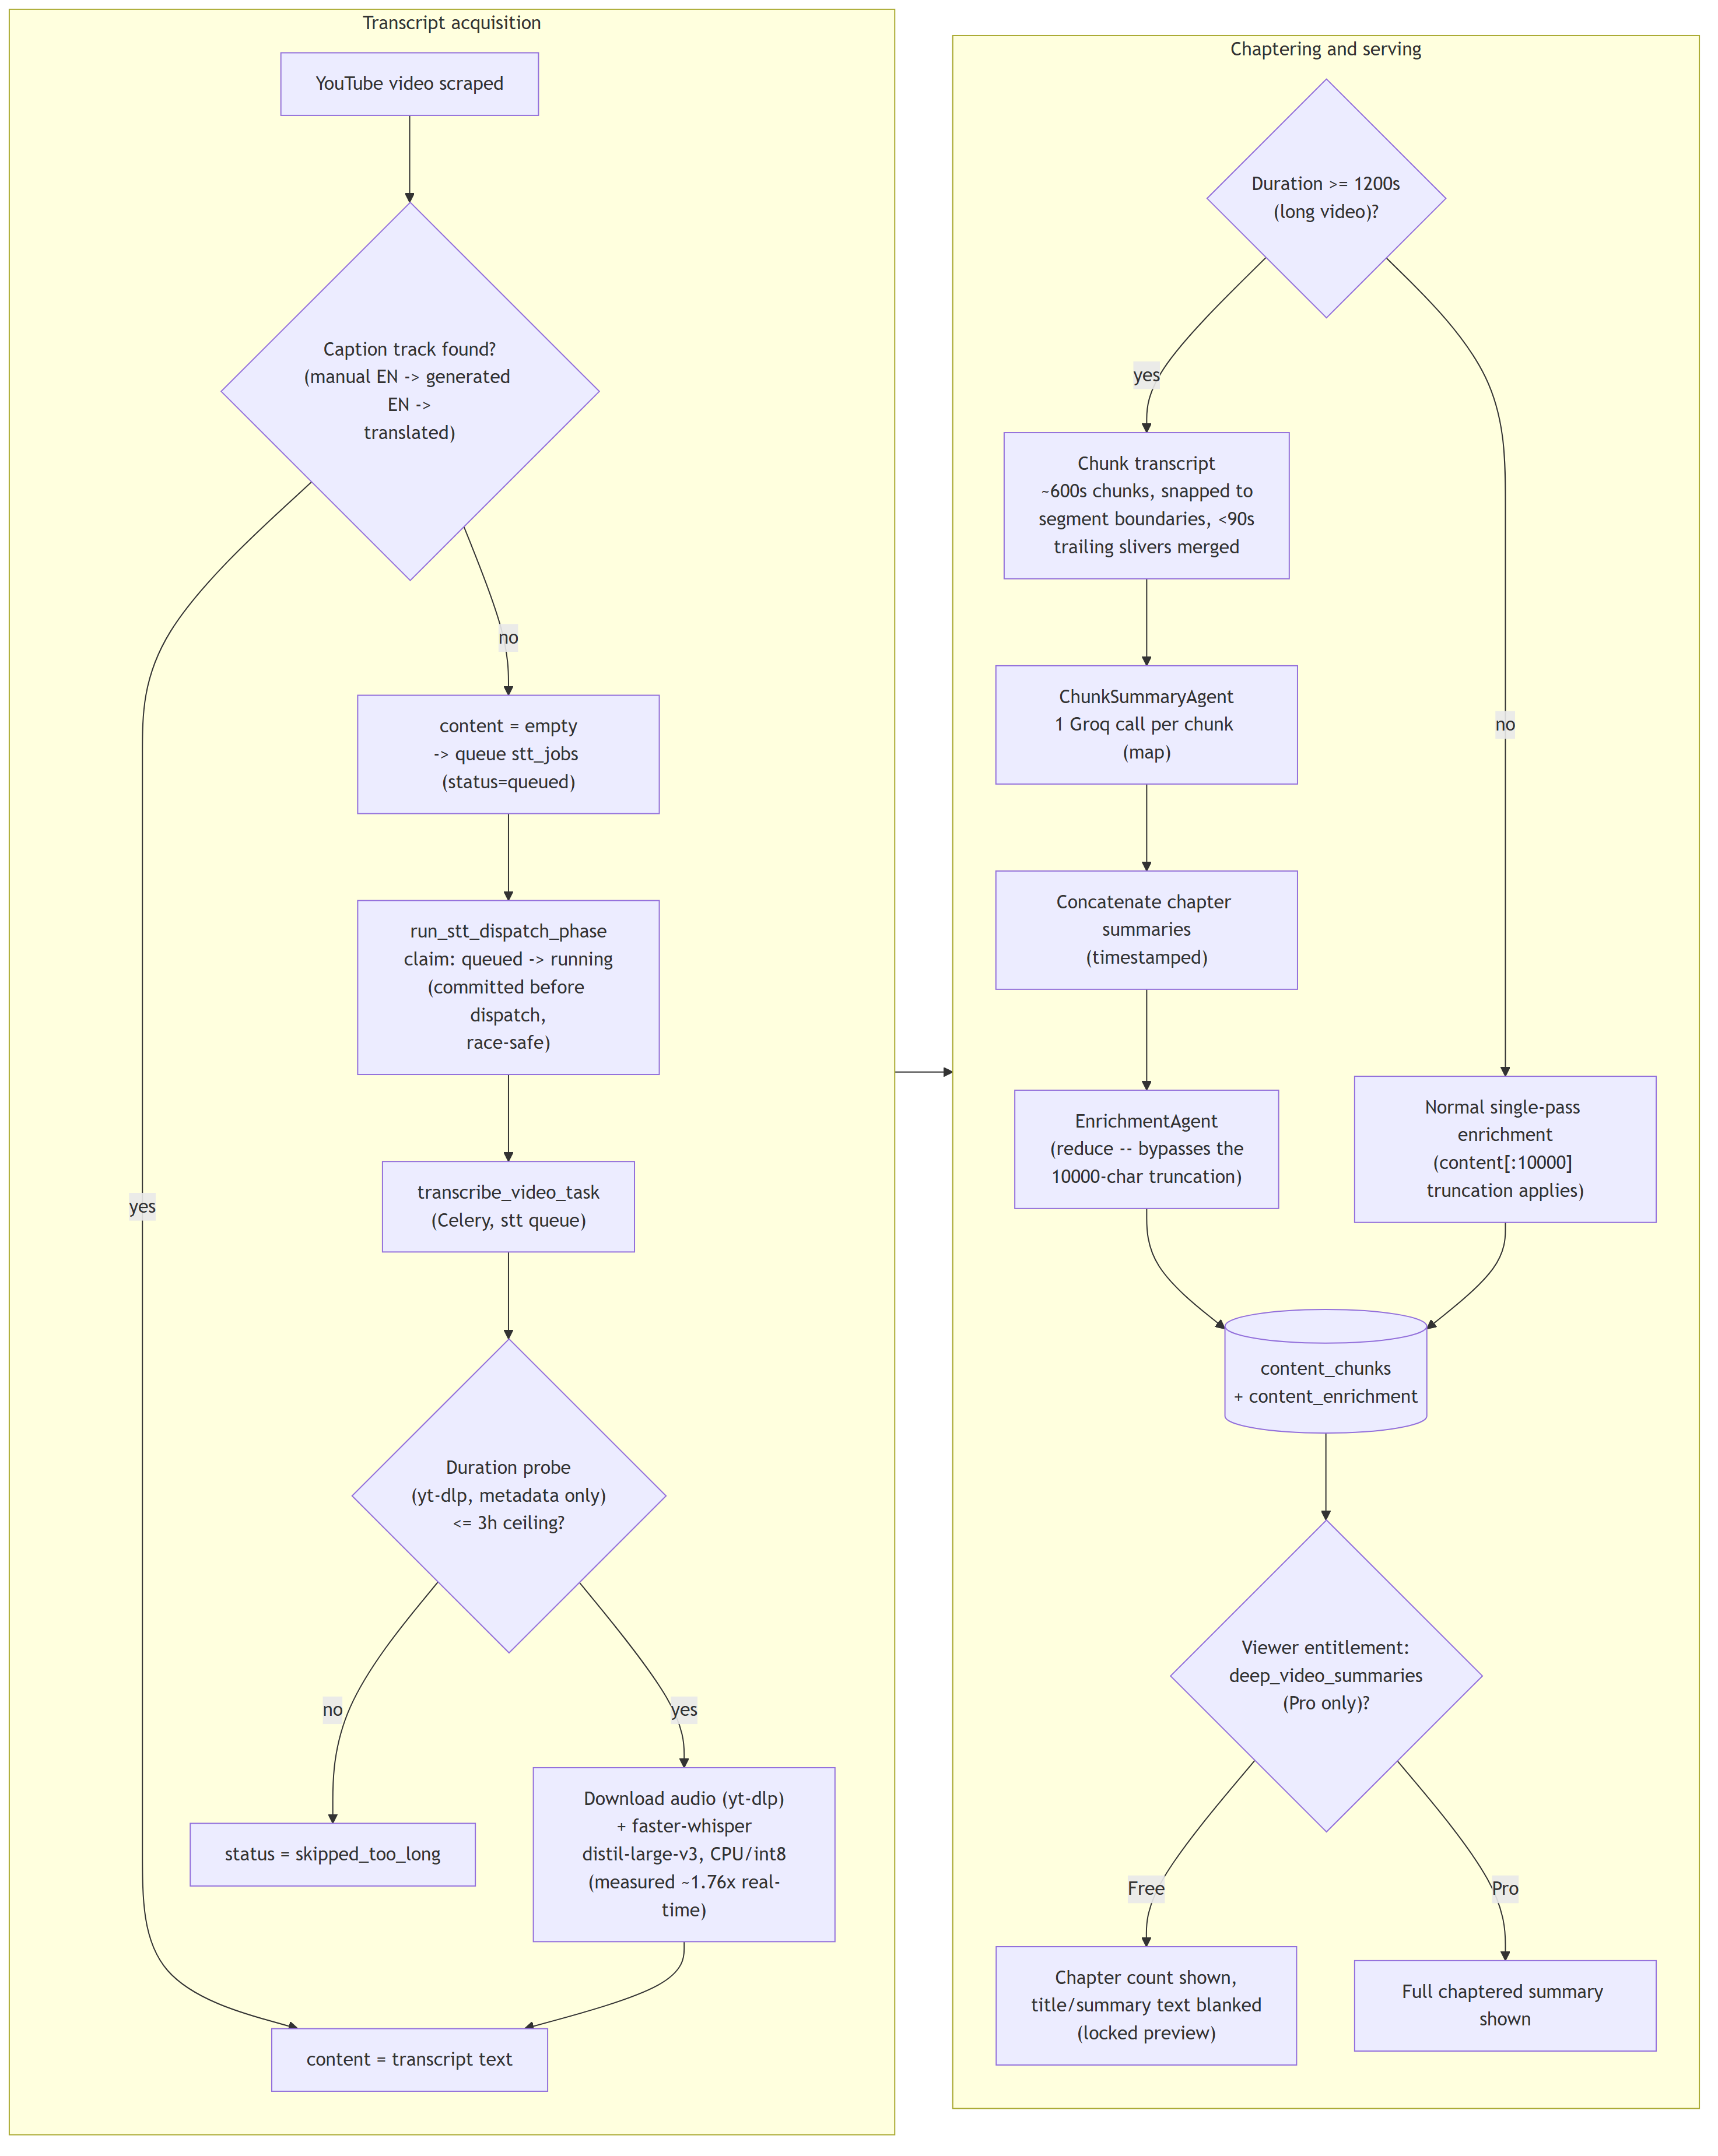
\includegraphics[width=0.85\textwidth,height=0.85\textheight,keepaspectratio]{figures/deep_media_pipeline.png}
\caption{Deep media processing pipeline: caption/STT transcript acquisition, duration-gated transcription, and long-video map-reduce chaptering.}
\label{fig:deep-media}
\end{figure}

Figure~\ref{fig:screenshot-video-chapters} shows the Pro-tier chaptered view produced by this pipeline: each chapter card carries the timestamp, title, and summary text produced by the per-chunk map step and left visible (unlike the Free-tier locked preview described in Section~\ref{sec:deep-media-entitlements}).

\begin{figure}[htbp]
\centering

\includegraphics[width=0.85\textwidth]{figures/screenshots/screenshot_video_chapters.png}
\caption{A video detail page showing the Pro-tier chaptered view, with per-chapter titles and summaries visible.}
\label{fig:screenshot-video-chapters}
\end{figure}
